\documentclass[a4j,titlepage]{jarticle}
\usepackage[dvipdfmx]{graphicx}
\usepackage{ascmac}
\usepackage{url}


\title{居酒屋検索システム\\
ユーザインターフェース設計書\\
第0版}
\author{株式会社Spirytus}
\date{\today}

\begin{document}
\maketitle
\tableofcontents

\section{一般ユーザの画面遷移}



まずトップ画面より、お酒の種類、味、アルコール度数から居酒屋を検索できる画面(¥ref{fig:図1})を表示する。



またタブ画面内において、高知県の代表的なお酒の説明を掲載する。



タブ画面外では高知県のお土産ベスト3を紹介し、各お土産の写真や説明を適宜記載する。



また高知県のイベント情報欄を作成し、月ごと(もしくは年間表)で高知県のイベント情報を記載する。



\begin {figure}[!htbp]
    \begin{center}
    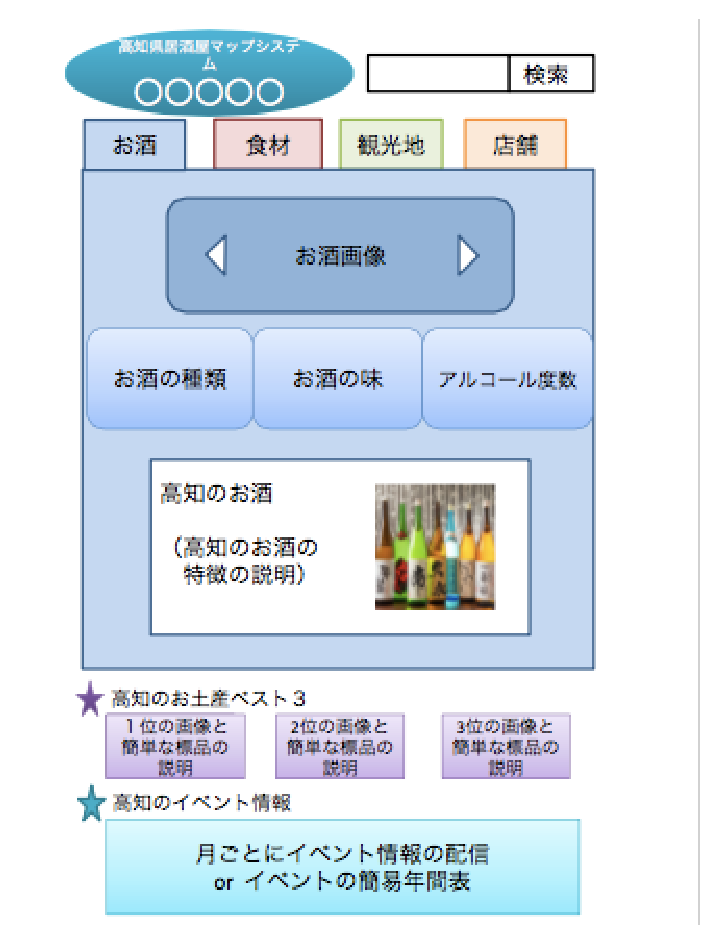
\includegraphics [height=12cm, width=10cm]{1.eps}
    \caption {お酒から居酒屋を検索する画面}
    \label {fig:1}
    \end{center}
\end {figure}


¥ref{fig:図1}の画面より「お酒の種類」をクリックすることで、全てのお酒の種類が表示される画面(¥ref{fig:図2})に遷移する。
\clearpage
\begin {figure}[!htbp]
    \begin{center}
    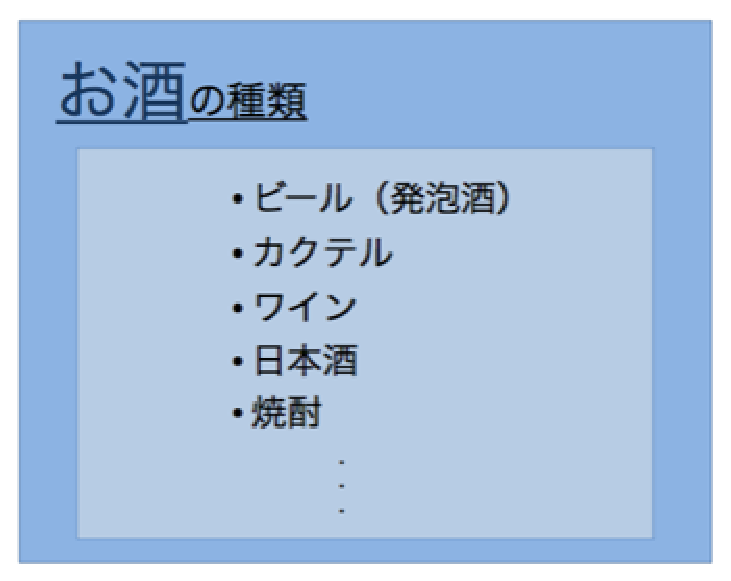
\includegraphics [height=7cm, width=7cm]{2.eps}
    \caption {お酒の種類を表示した画面}
    \label {fig:2}
    \end{center}
\end {figure}


¥ref{fig:図2}の画面よりお酒の種類(ビールやカクテル等)をクリックすることで、選択した種類に当てはまる酒名を表示する画面(¥ref{fig:図3})に遷移する。(ここでは例として「焼酎」を選択)

\begin {figure}[!htbp]
    \begin{center}
    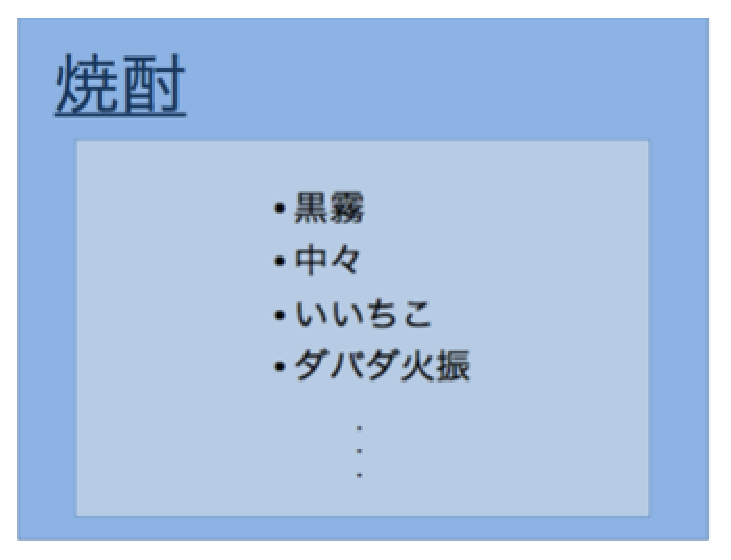
\includegraphics [height=7cm, width=7cm]{3.eps}
      \caption {選択した種類に当てはまる酒名を表示した画面}
    \label {fig:3}
    \end{center}
\end {figure}
¥ref{fig:図3}の画面より酒名をクリックすることで、選択したお酒の詳細情報およびそのお酒を扱っている店舗の一覧表が表示される画面(¥ref{fig:図4})に遷移する。(ここでは例として「ダバダ火振」を選択)
\clearpage
\begin {figure}[!htbp]
    \begin{center}
    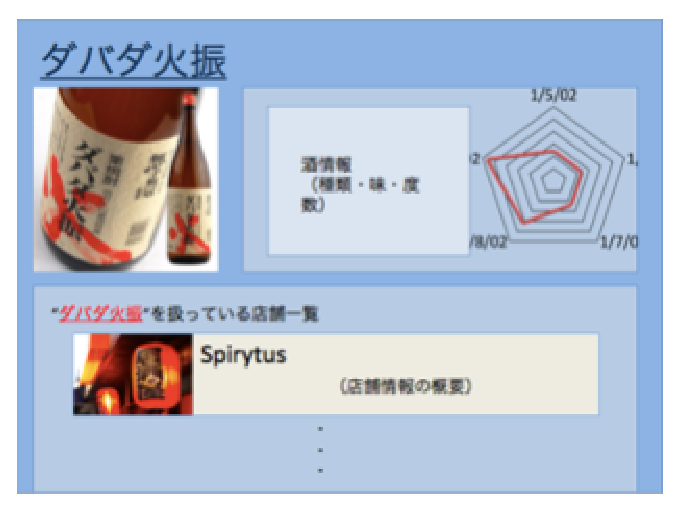
\includegraphics [height=7cm, width=7cm]{4.eps}
    \caption {お酒の詳細情報およびそのお酒を扱っている店舗の一覧が表示される画面}
    \label {fig:4}
    \end{center}
\end {figure}



¥ref{fig:図4}の画面より店舗名をクリックすることで、選択した店舗の詳細情報が表示される画面(¥ref{fig:図5})に遷移する。

\begin {figure}[!htbp]
    \begin{center}
    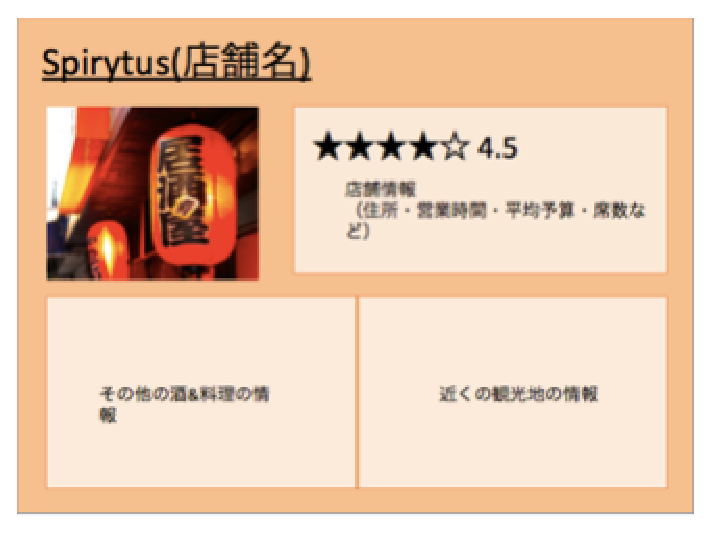
\includegraphics [height=7cm, width=7cm]{5.eps}
    \caption {店舗の詳細情報が表示される画面}
    \label {fig:5}
    \end{center}
\end {figure}

¥ref{fig:図1}の画面より「お酒の味」をクリックすることで、全てのお酒の味が表示される画面(¥ref{fig:図6})に遷移する。
\clearpage
\begin {figure}[!htbp]
    \begin{center}
    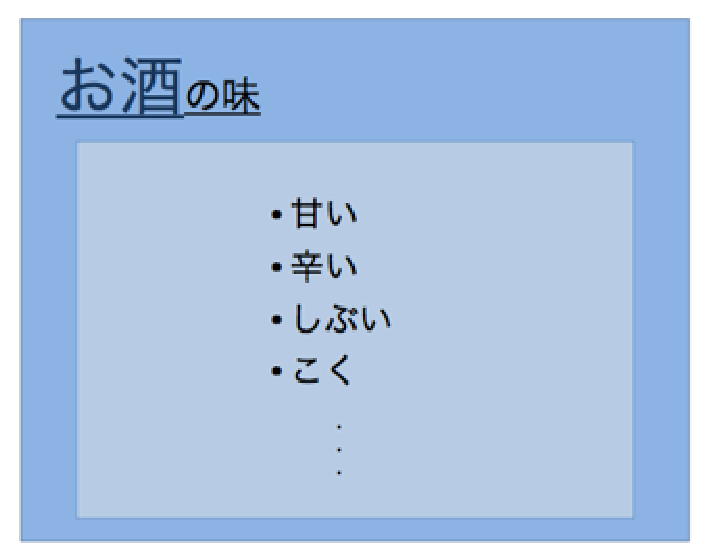
\includegraphics [height=7cm, width=7cm]{6.eps}
    \caption {お酒の味が表示される画面}
    \label {fig:6}
    \end{center}
\end {figure}
¥ref{fig:図6}の画面よりお酒の味(甘いや辛い等)をクリックすることで、選択した味に当てはまる酒名を表示する画面(¥ref{fig:図7})に遷移する(ここでは例として「しぶい」を選択)。



その後酒名を選択することで、選択したお酒の詳細情報画面(¥ref{fig:図4})に遷移する。

\begin {figure}[!htbp]
    \begin{center}
    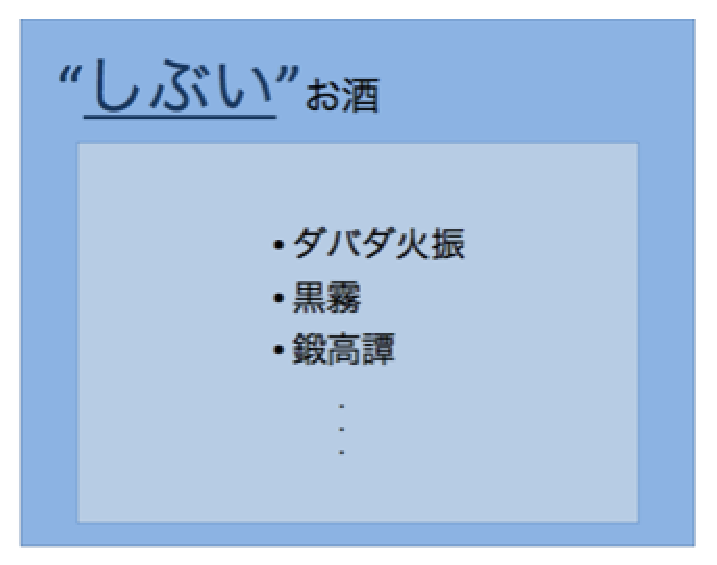
\includegraphics [height=7cm, width=7cm]{7.eps}
    \caption {選択したお酒の味に当てはまる酒名を表示する画面}
    \label {fig:7}
    \end{center}
\end {figure}



次にトップ画面より、高知の食材(魚、肉、野菜)、郷土料理から居酒屋を検索できる画面(¥ref{fig:図8})を表示する。



またタブ画面内において、高知県の代表的な食材の説明を掲載する。



タブ画面外の高知県のお土産ベスト3および、高知県のイベント情報は、お酒から検索できる画面と同様で変化しない。
\clearpage
\begin {figure}[!htbp]
    \begin{center}
    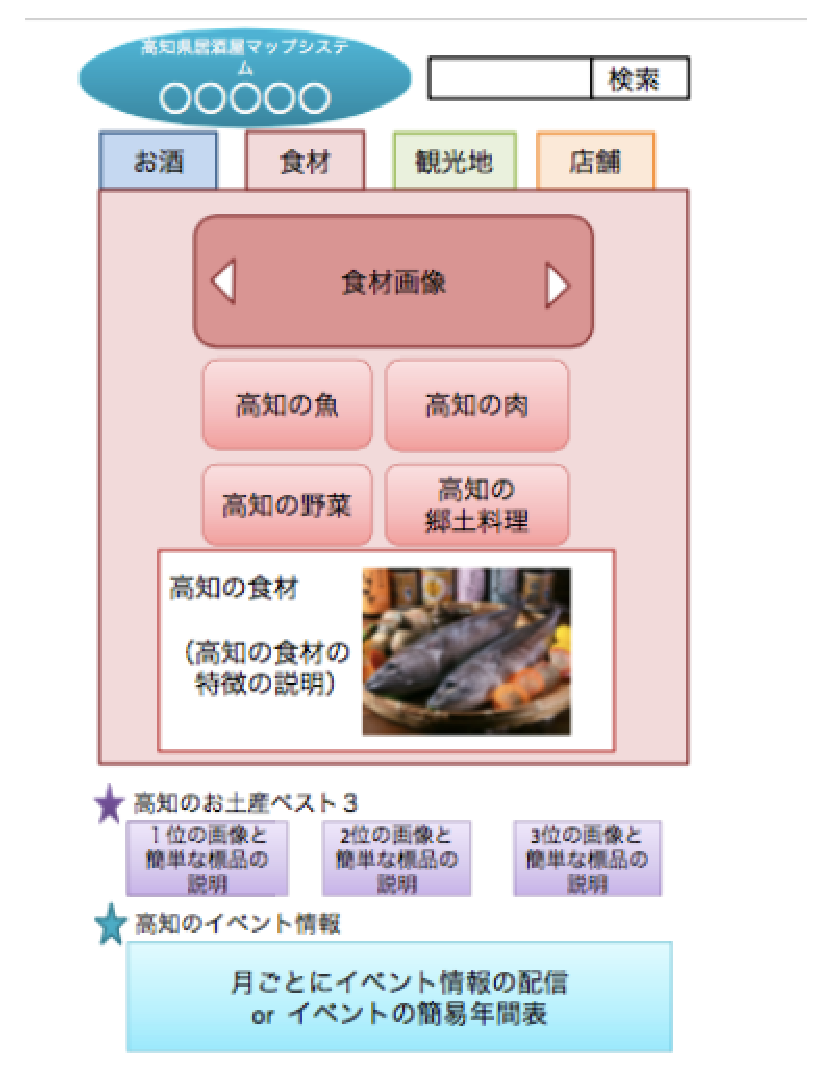
\includegraphics [height=12cm, width=10cm]{8.eps}
    \caption {高知の食材および郷土料理から居酒屋を検索する画面}
    \label {fig:8}
    \end{center}
\end {figure}



¥ref{fig:図8}の画面より、例として「高知の野菜」をクリックすることで、有名な(出荷量が多い、知名度の高い)高知の野菜が表示される画面(¥ref{fig:図9})に遷移する。
\clearpage
\begin {figure}[!htbp]
    \begin{center}
    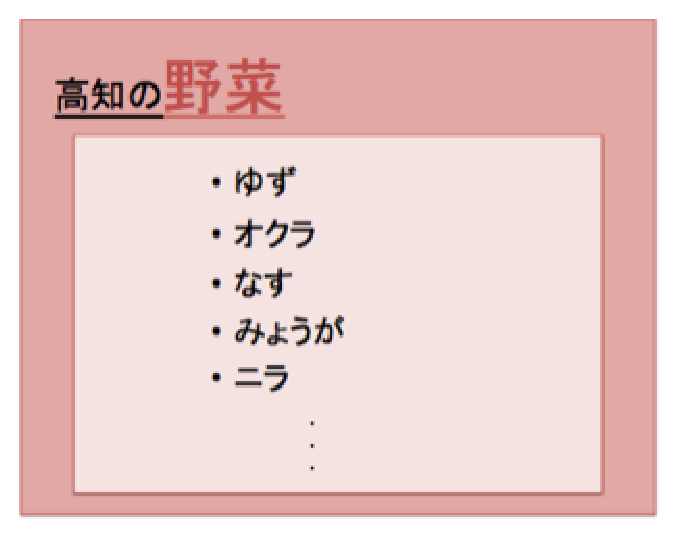
\includegraphics [height=7cm, width=7cm]{9.eps}
    \caption {高知県の野菜を表示する画面}
    \label {fig:9}
    \end{center}
\end {figure}



¥ref{fig:図9}の画面より、表示された野菜名をクリックすることで、選択した野菜の説明およびその食材がどのような料理に扱われているのかを示した画面(¥ref{fig:図10})が表示される(ここでは例として「ゆず」を選択)。



またこの画面から、この野菜を扱った料理を提供している居酒屋を検索することができる。



\begin {figure}[!htbp]
    \begin{center}
    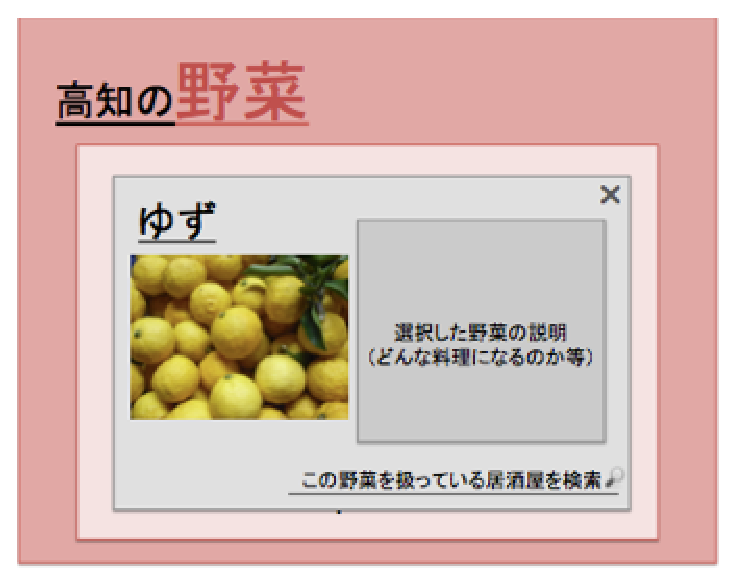
\includegraphics [height=7cm, width=7cm]{10.eps}
      \caption {選択した野菜の説明画面}
    \label {fig:10}
    \end{center}
\end {figure}



¥ref{fig:図10}の画面より、「この野菜を扱っている居酒屋を検索」をクリックすることで、選択した野菜を扱っている居酒屋を全て表示する画面(¥ref{fig:図11})に遷移する。



その後、気になる居酒屋を選択しクリックすることで、その店舗の詳細情報を表示する画面(¥ref{fig:図5})へ遷移する。
\clearpage
\begin {figure}[!htbp]
    \begin{center}
    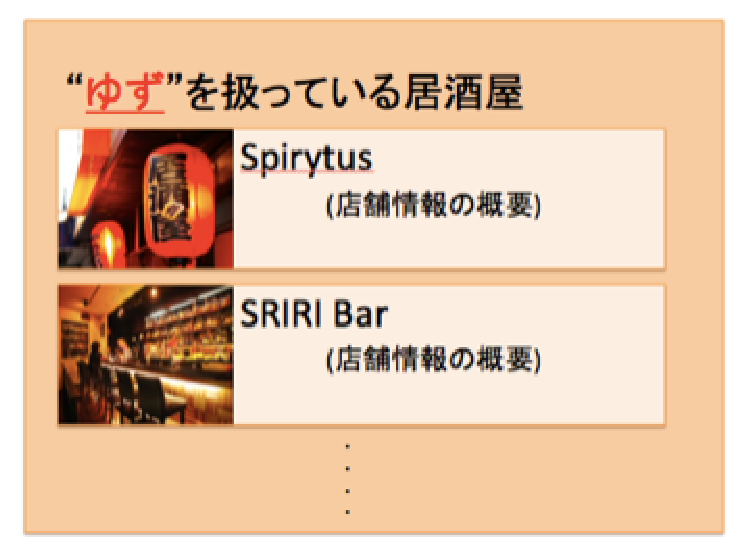
\includegraphics [height=10cm, width=10cm]{11.eps}
    \caption {選択した野菜を扱っている店舗一覧を表示する画面}
    \label {fig:11}
    \end{center}
\end {figure}

※高知の魚、肉、郷土料理においても上記と同じ画面遷移を行う。
次にトップ画面より、高知の観光地から居酒屋を検索できる画面(¥ref{fig:図12})を表示する。



まず高知の観光地ベスト5として、観光地を5箇所掲載する。



またタブ画面内において、高知県の代表的な観光地の説明を掲載する。



タブ画面外の高知県のお土産ベスト3および、高知県のイベント情報は、お酒から検索できる画面と同様で変化しない。
\clearpage
\begin {figure}[!htbp]
    \begin{center}
    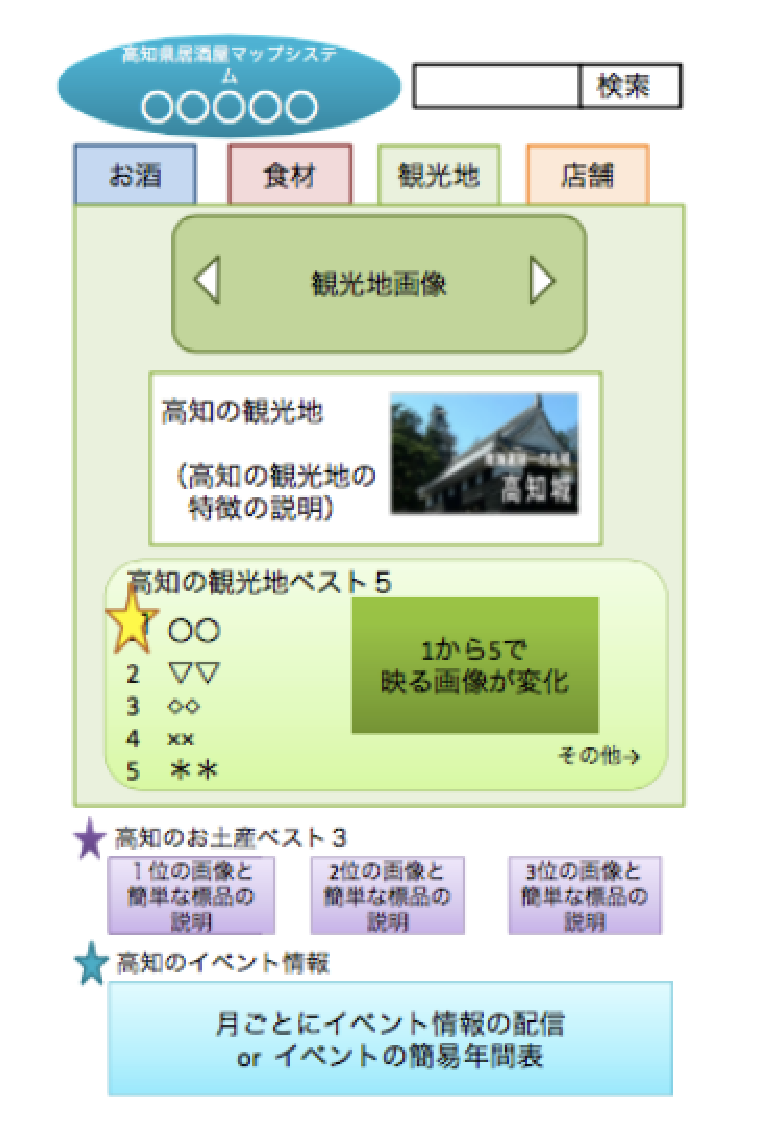
\includegraphics [height=12cm, width=10cm]{12.eps}
    \caption {観光地から居酒屋を検索する画面}
    \label {fig:12}
    \end{center}
\end {figure}

¥ref{fig:図12}の画面より、高知の観光地ベスト5欄内の「詳細」をクリックすることで、全ての観光地が表示される画面(¥ref{fig:図13})に遷移する。

(ベスト5の観光地はランク(または色分け)をつけ、それ以外は番号をつけない)
\clearpage
\begin {figure}[!htbp]
    \begin{center}
    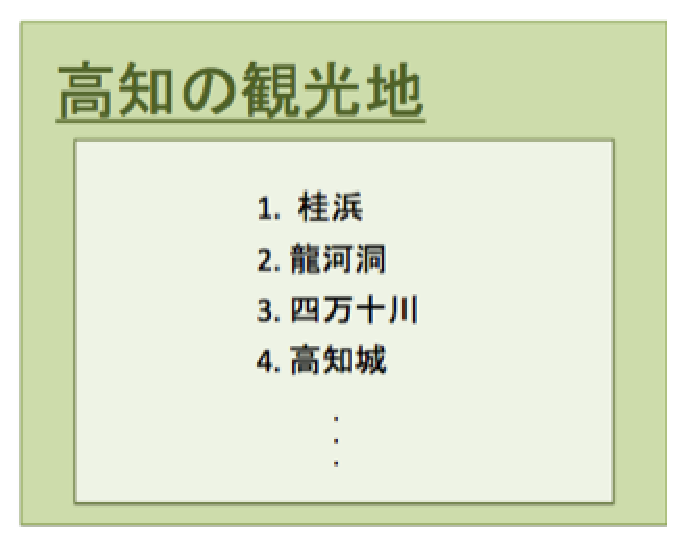
\includegraphics [height=7cm, width=7cm]{13.eps}
    \caption {全ての観光地を表示する画面}
    \label {fig:13}
    \end{center}
\end {figure}



¥ref{fig:図13}の画面より、表示された観光地名をクリックすることで、選択した観光地の詳細情報が表示される(ここでは例として「桂浜」を選択)。



またこの画面から、この観光地周辺の居酒屋を検索することができる。



\begin {figure}[!htbp]
    \begin{center}
    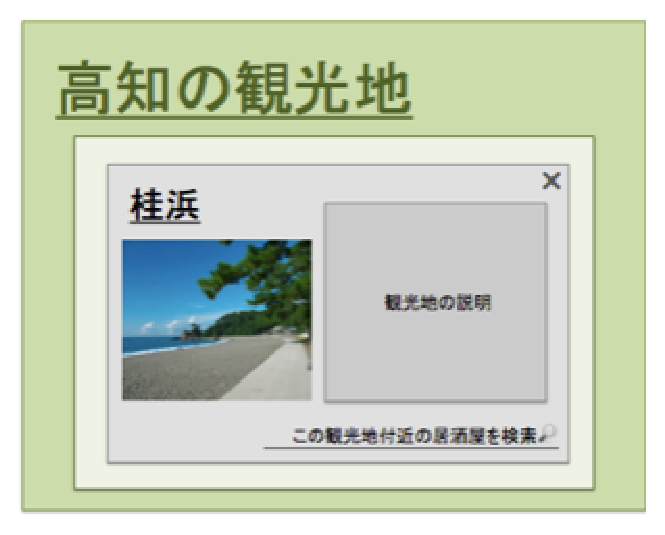
\includegraphics [height=7cm, width=7cm]{14.eps}
    \caption {選択した観光地の説明画面}
    \label {fig:14}
    \end{center}
\end {figure}



¥ref{fig:図14}の画面より、「この観光地付近の居酒屋を検索」をクリックすることで、選択した観光地周辺の居酒屋を全て表示する画面(¥ref{fig:図15})に遷移する。



その後、気になる居酒屋を選択しクリックすることで、その店舗の詳細情報を表示する画面(¥ref{fig:図5})へ遷移する。
\clearpage
\begin {figure}[!htbp]
    \begin{center}
    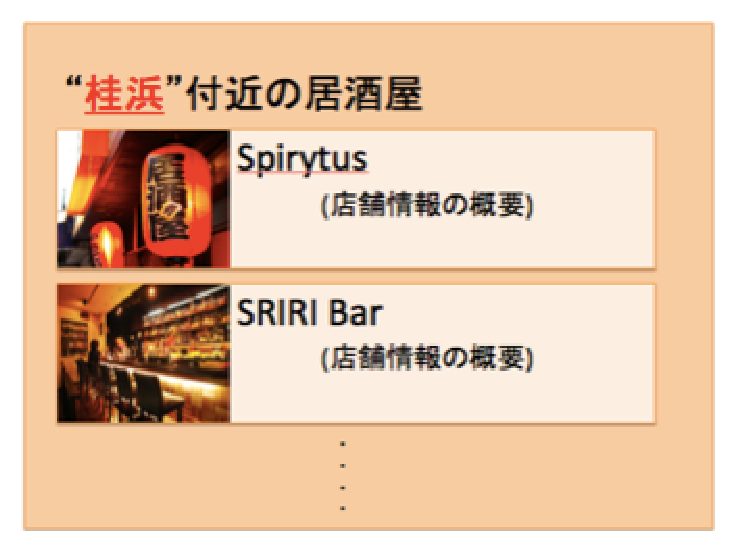
\includegraphics [height=7cm, width=7cm]{15.eps}
    \caption {選択した観光地周辺の居酒屋一覧表を表示する画面}
    \label {fig:15}
    \end{center}
\end {figure}



次にトップ画面より、店舗の特徴から居酒屋を検索できる画面(¥ref{fig:図16})を表示する。



具体的にはその店舗の所在地や平均予算から居酒屋を検索することができる。



タブ画面外の高知県のお土産ベスト3および、高知県のイベント情報は、お酒から検索できる画面と同様で変化しない。
\clearpage
\begin {figure}[!htbp]
    \begin{center}
    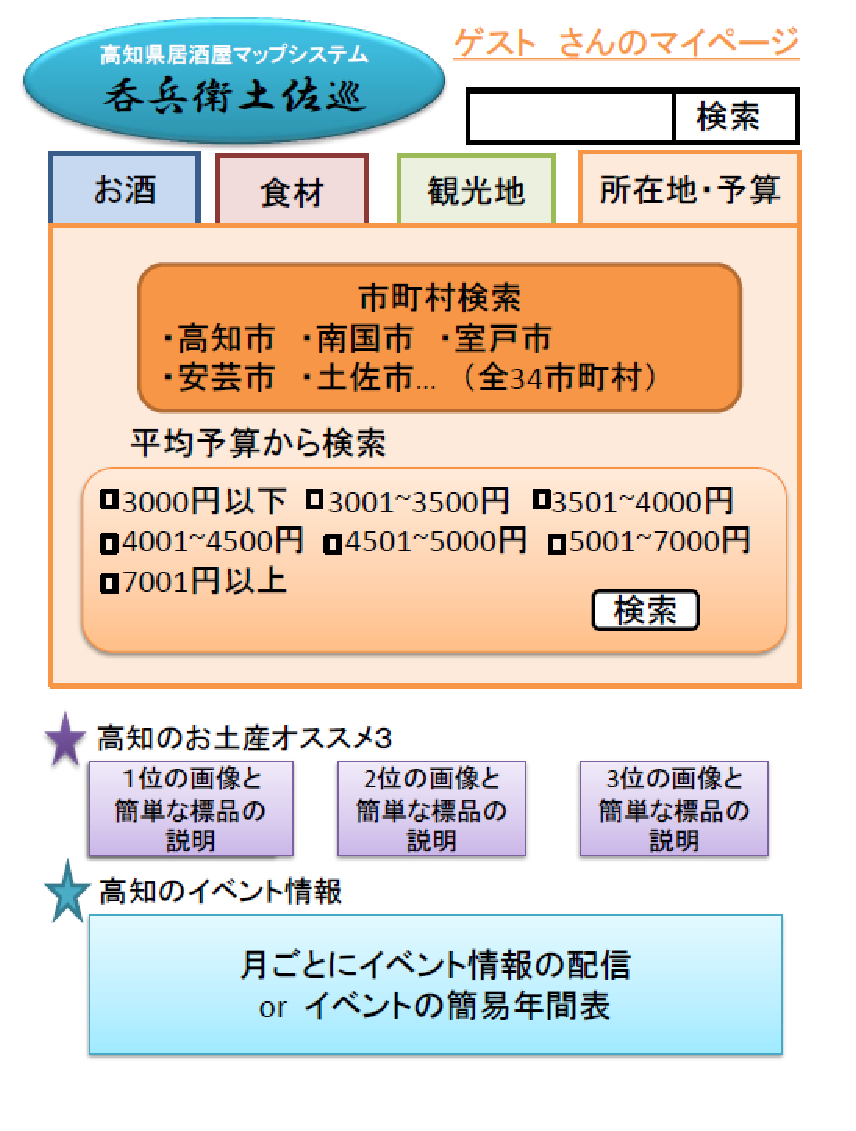
\includegraphics [height=12cm, width=10cm]{16.eps}
    \caption {店舗の特徴から}
    \label {fig:16}
    \end{center}
\end {figure}



¥ref{fig:図16}の画面の市町村検索から、例として「高知市」をクリックすることで、高知市に所在する居酒屋一覧表を表示する画面(¥ref{fig:図17})に遷移する。



その後、気になる居酒屋を選択しクリックすることで、その店舗の詳細情報を表示する画面(¥ref{fig:図5})へ遷移する。
\clearpage

\begin {figure}[!htbp]
    \begin{center}
    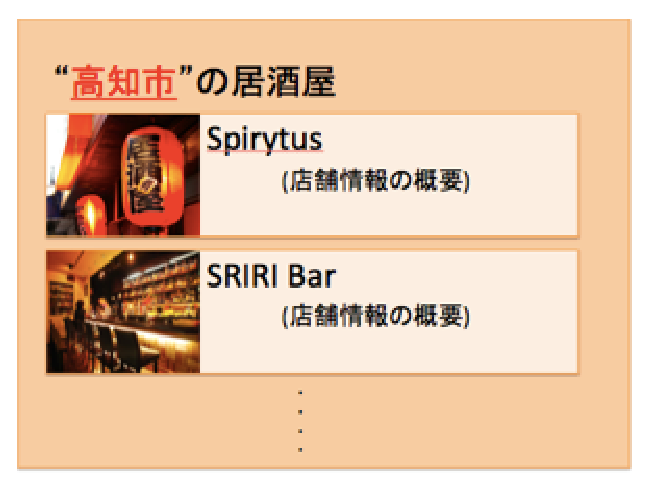
\includegraphics [height=7cm, width=7cm]{17.eps}
      \caption {選択した市町村に所在する居酒屋の一覧表を表示する画面}
    \label {fig:17}
    \end{center}
\end {figure}



¥ref{fig:図16}の画面の平均予算検索から、例として「3000円以下」をクリックすることで、平均予算が3000円以下である居酒屋一覧表を表示する画面(¥ref{fig:図18})に遷移する。



その後、気になる居酒屋を選択しクリックすることで、その店舗の詳細情報を表示する画面(¥ref{fig:図5})へ遷移する。
\clearpage

\begin {figure}[!htbp]
    \begin{center}
    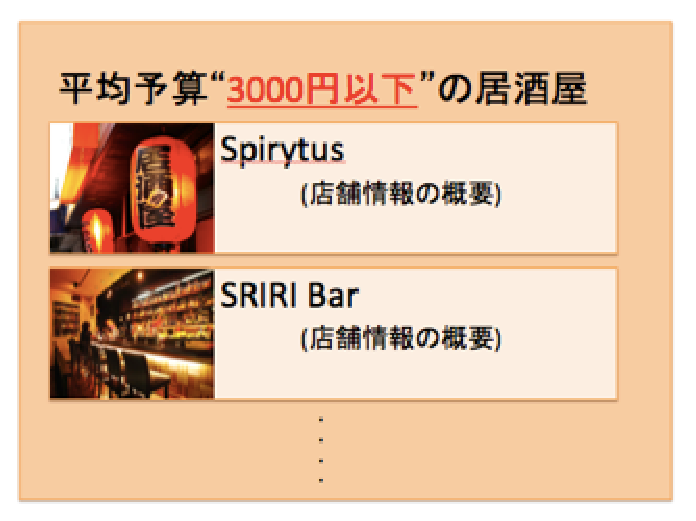
\includegraphics [height=7cm, width=7cm]{18.eps}
    \caption {選択した平均予算に当てはまる居酒屋の一覧表を表示する画面}
    \label {fig:18}
    \end{center}
\end {figure}



上記で説明した一般ユーザの画面遷移を全体的にまとめたものを以下に示す。



\begin {figure}[!htbp]
    \begin{center}
    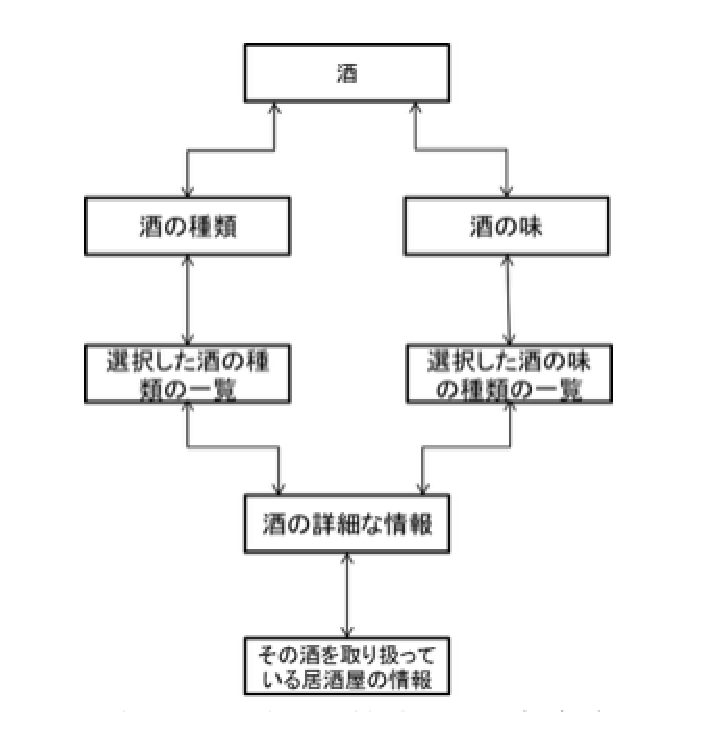
\includegraphics [height=10cm, width=10cm]{19.eps}
    \caption {お酒から居酒屋を検索する画面遷移の全体図}
    \label {fig:19}
    \end{center}
\end {figure}



\begin {figure}[!htbp]
    \begin{center}
    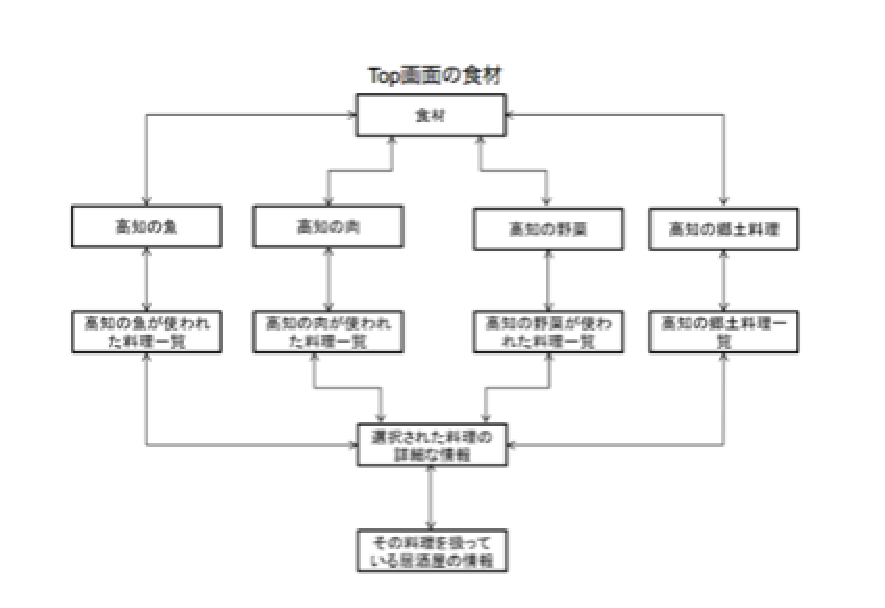
\includegraphics [height=10cm, width=10cm]{20.eps}
    \caption {高知の食材から居酒屋を検索する画面遷移の全体図}
    \label {fig:20}
    \end{center}
\end {figure}


\begin {figure}[!htbp]
    \begin{center}
    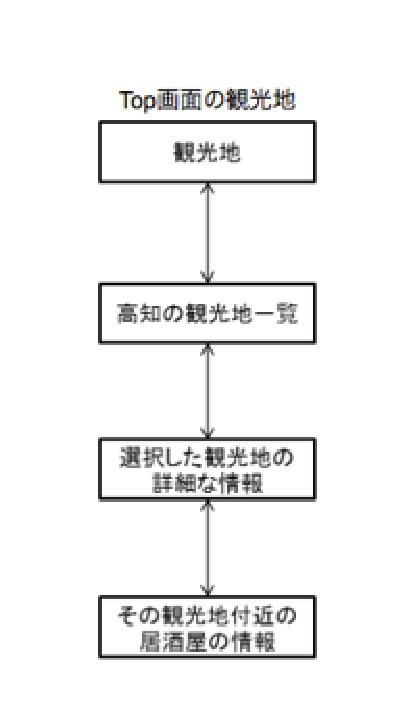
\includegraphics [height=10cm, width=10cm]{21.eps}
    \caption {高知の観光地から居酒屋を検索する画面遷移の全体図}
    \label {fig:21}
    \end{center}
\end {figure}

\clearpage

\section{ユーザ登録画面}
 ユーザ登録フォーム画面より、高知県居酒屋マップシステムを使用するために必要なE-mailアドレス、アカウント名、パスワードを入力する画面(¥ref{fig:図22})を表示する。



パスワードは間違いがないか確認するため、2回入力する欄がある。



全てを入力し終えた後「登録」をクリックすることで、登録完了画面(¥ref{fig:図23})に遷移する。




\begin {figure}[!htbp]
    \begin{center}
    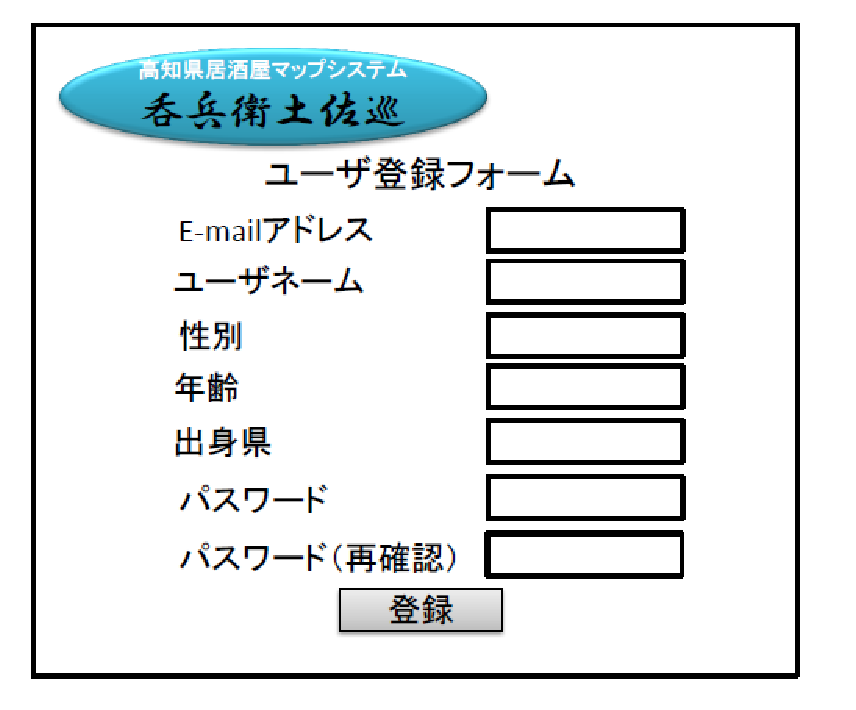
\includegraphics [height=7cm, width=7cm]{22.eps}
    \caption {ユーザ登録フォーム}
    \label {fig:22}
    \end{center}
\end {figure}



\begin {figure}[!htbp]
    \begin{center}
    
\includegraphics [height=7cm, width=7cm]{23.eps}
    \caption {ユーザ登録完了画面}
    \label {fig:23}
    \end{center}
\end {figure}



¥ref{fig:図23}の画面より「トップ画面へ」をクリックすることで、トップ画面(¥ref{fig:図1})に遷移する。



\begin {figure}[!htbp]
    \begin{center}
    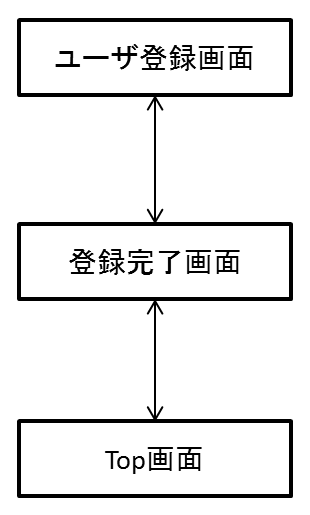
\includegraphics [height=7cm, width=7cm]{24.eps}
    \caption {ユーザ登録の画面遷移}
    \label {fig:24}
    \end{center}
\end {figure}
\clearpage
\section{店舗側の画面遷移}


 始めに店舗側は、店舗側の新規登録フォーム画面(¥ref{fig:図2})により店舗の登録を申請する。



E-mailアドレスを入力した後、「登録申請」をクリックすることで、店舗登録の申請が完了したことを知らせる画面(¥ref{fig:図26})に遷移する。



\begin {figure}[!htbp]
    \begin{center}
    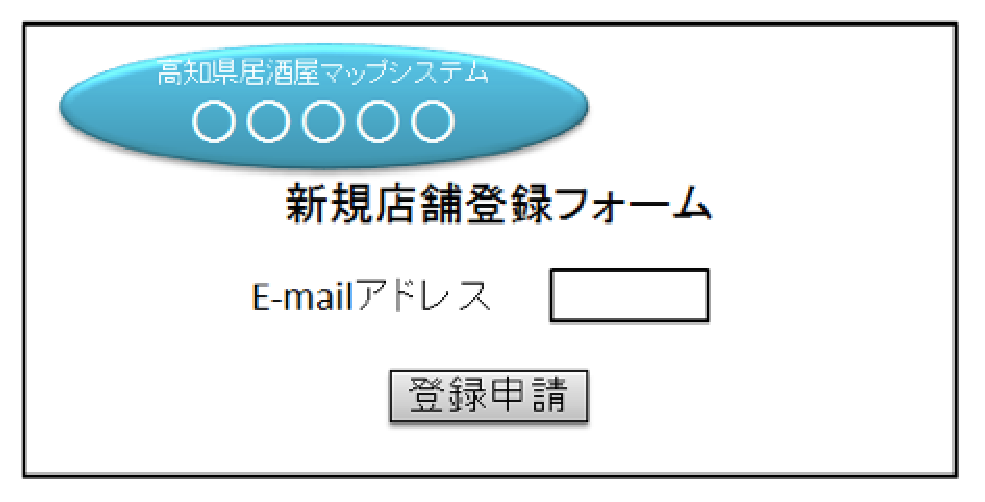
\includegraphics [height=10cm, width=10cm]{25.eps}
      \caption {店舗側登録フォーム}
    \label {fig:25}
    \end{center}
\end {figure}



\begin {figure}[!htbp]
    \begin{center}
    
\includegraphics [height=10cm, width=10cm]{26.eps}
    \caption {店舗登録申請完了画面}
    \label {fig:26}
    \end{center}
\end {figure}


\clearpage
ログイン画面(¥ref{fig:図27})では、店舗が情報を編集する画面にログインするための画面を表示する。



登録している店舗はE-mailアドレスとパスワードを入力した後「ログイン」をクリックすることで、店舗の情報を編集する画面(¥ref{fig:図2})に遷移する。



ログインに失敗した場合、「(E-mailアドレス、またはパスワードが間違っています)」の文章が付け加わったログイン画面が表示される。



登録したい店舗は「こちら」をクリックすることで、店舗側の登録フォーム画面(¥ref{fig:図2})へ遷移する。



\begin {figure}[!htbp]
    \begin{center}
    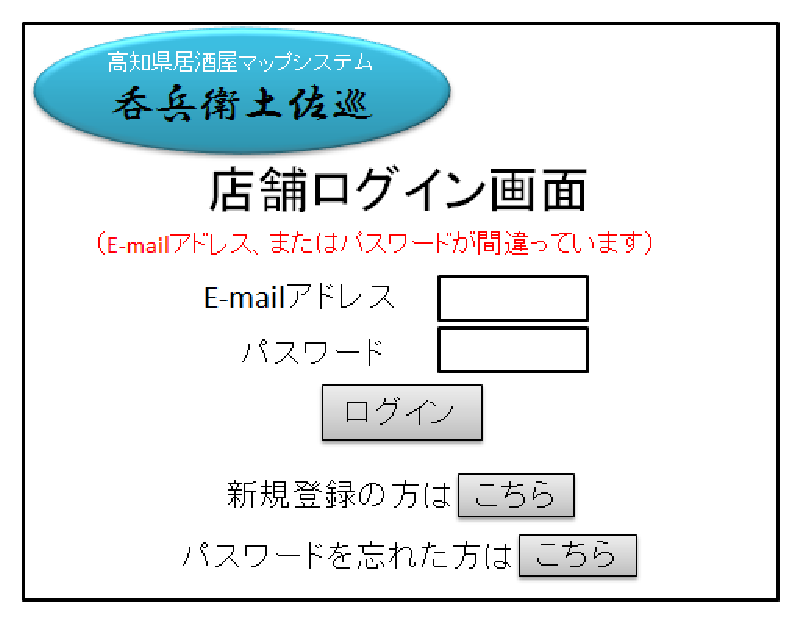
\includegraphics [height=10cm, width=10cm]{27.eps}
    \caption {店舗側のログイン画面}
    \label {fig:27}
    \end{center}
\end {figure}



\begin {figure}[!htbp]
    \begin{center}
    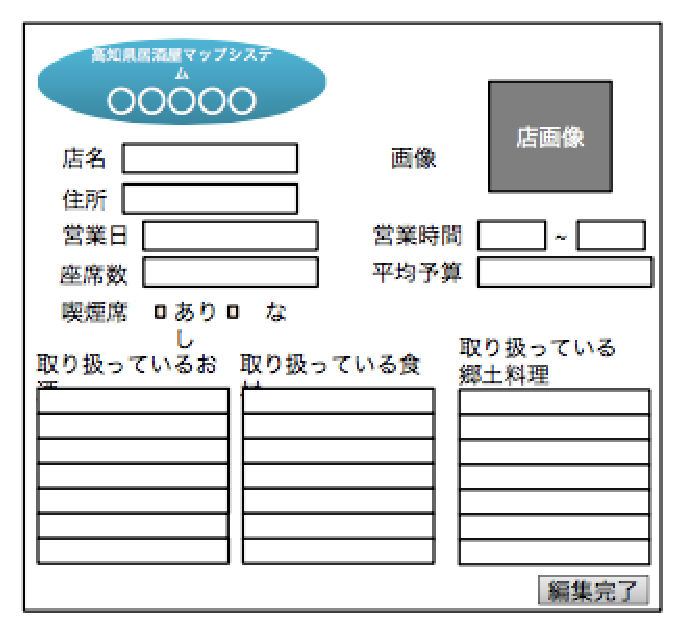
\includegraphics [height=10cm, width=10cm]{28.eps}
    \caption {店舗の情報編集画面}
    \label {fig:28}
    \end{center}
\end {figure}



\begin {figure}[!htbp]
    \begin{center}
    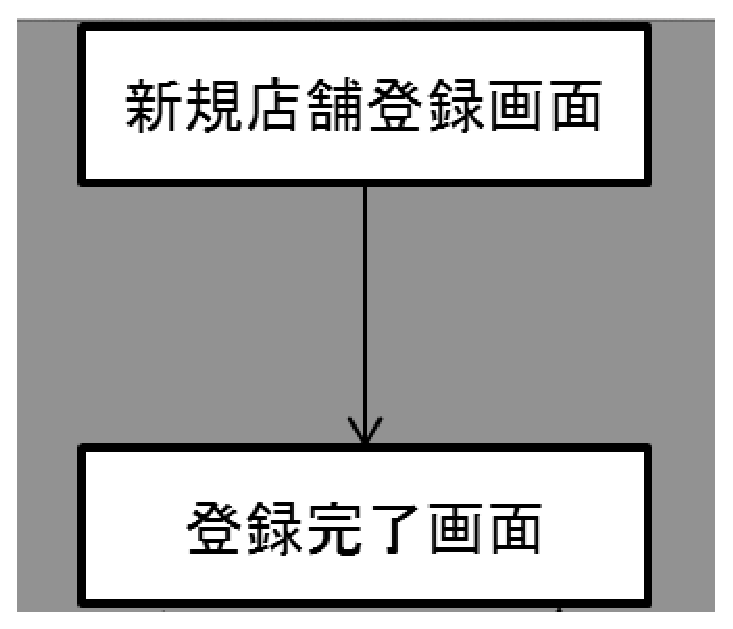
\includegraphics [height=10cm, width=10cm]{29.eps}
    \caption {店舗登録画面遷移図}
    \label {fig:29}
    \end{center}
\end {figure}
\clearpage
¥ref{fig:図28}では、店舗側に編集してもらう情報の記述欄とチェック欄を表示する。



全ての項目欄を記述後「編集確認」をクリックすることで、編集した内容を確認するプレビュー画面(¥ref{fig:図30})に遷移する。



\begin {figure}[!htbp]
    \begin{center}
    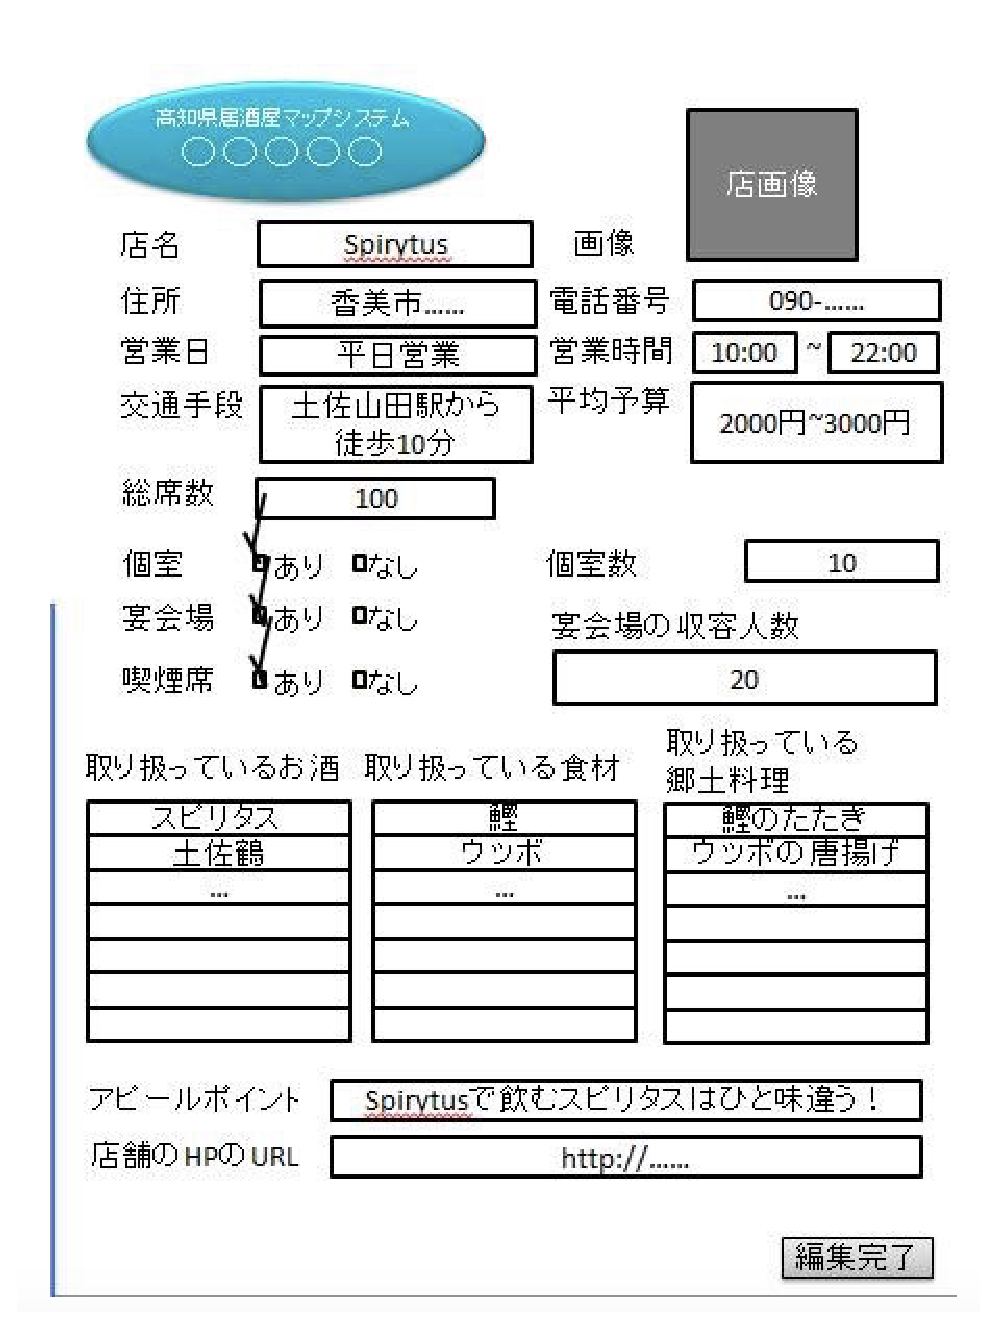
\includegraphics [height=10cm, width=10cm]{30.eps}
    \caption {プレビュー画面}
    \label {fig:30}
    \end{center}
\end {figure}


\clearpage
¥ref{fig:図30}では、¥ref{fig:図28}で編集した情報を再表示する。



編集した情報に間違いがないことを確認したのち「編集完了」をクリックすることで、編集を完了したことを伝える画面(¥ref{fig:図31})へ遷移する。



\begin {figure}[!htbp]
    \begin{center}
    
\includegraphics [height=10cm, width=10cm]{31.eps}
    \caption {編集完了画面}
    \label {fig:31}
    \end{center}
\end {figure}



¥ref{fig:図29}は、店舗情報の編集を完了したことを知らせる画面を表示する。



「編集画面」をクリックすることで、再び店舗の編集画面(¥ref{fig:図28})へ遷移する。
\clearpage

上記で説明した店舗側の画面遷移を全体にまとめたものを以下に示す。
\begin {figure}[!htbp]
    \begin{center}
    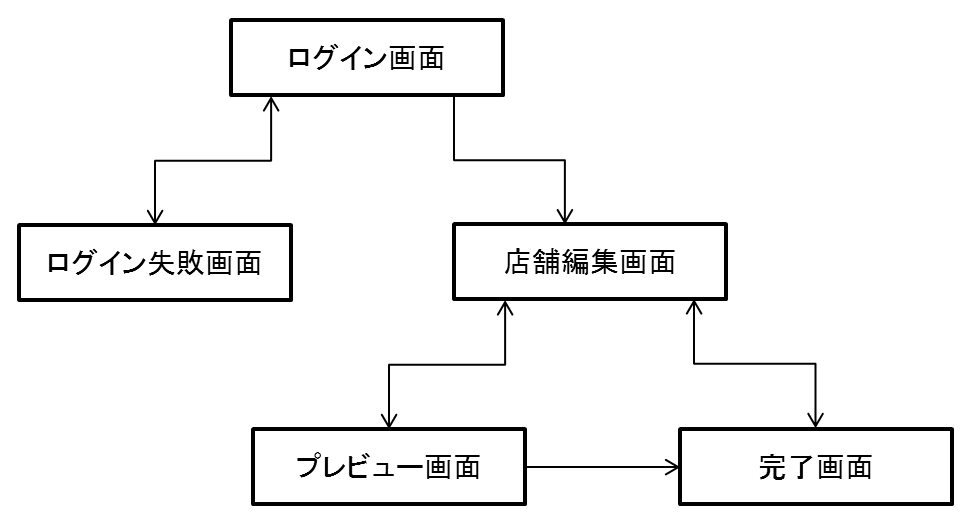
\includegraphics [height=10cm, width=10cm]{32.eps}
    \caption {店舗側の情報遷移図}
    \label {fig:32}
    \end{center}
\end {figure}

\end{document}
